\documentclass{article}
\usepackage[utf8]{inputenc}
\usepackage[pdftex]{graphicx}
\graphicspath{{./fig/}}

\title{Topic Modeling Library and Framework User Guide}
\author{Avanesov Valeriy\\Kozlov Ilya}
\date{\today}

\usepackage{natbib}
\usepackage{hyperref}
\begin{document}

\maketitle

\section{Input}
    The aim of this project is to provide flexible and simple library and framework for topic modeling.
    The main properties of this project:
    \begin{itemize}
	\item Ability to apply user's defined regularizer, sparsifier and stopping criteria.
	\item Ability to use multilingual topic modeling. 
    \end{itemize}
    The paper is organized as follow: section \ref{intro} contain a quick introduction on topic modeling,
    \ref{quickStart} describe how to start project, without description of details of implementation. These two sections should allow you
    to use model LDA or PLSA in a simple use\--causes. The fallowing section describes a details of implementation and it necessary for
    deeper understanding of project structure and implementation of your own regularizer, sparsifier and other stuff.
    Section \ref{projectStructure} describe structure of project, section \ref{regularizer} describe regularizers and explain how to implement you
    own regularizer, section \ref{sparsifier} describe what sparsifier is and how to implement you own sparsifier. Section \ref{stoppingCriteria}
    describe how to define that we do enough iteration of EM\--algorithm. Section \ref{multilingual} describe how to use model in case of a multilingual
    texts. 

\clearpage	\section{Introduction to the topic modeling}  \label{intro}    \subsection{Generative model}
\label{generativeModel}
    In topic modeling every document viewed as mixture of topics. Each topic is a multinomial distribution on words,
    so generation model may be defined as follow:
    \begin{itemize} \label{generation}
	\item For every position in document $d$ i.i.d choose topic $t$ from distribution of topics by document
	\item Choose word $w$ from topic $t$
    \end{itemize}
    \begin{figure}[!ht]
	\caption{Graphical representation of PLSA generative process}
	\begin{minipage}{\textwidth}
	    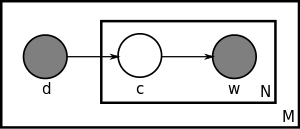
\includegraphics[width=0.55\linewidth]{plsa}
	\end{minipage}
    \end{figure}
    The aim of topic modeling is to recover topics and distribution of document by topics.
    \subsubsection{Polylingual topic model}
	Suppose one has a collection of documents on different languages. We have a prior knowledge that some of the
	documents (or all of them) are written on the same topic but in different languages (for example one document may be a translation of another).
	Wikipedia may be considered as a source of this type of data. It leads us to a polylingual topic modeling \cite{polylingual}.
	In this model we assume that every topic is a set of multinomial distributions, one per language. Also we assume that
	every document may hold more than one set of words, so we represent document as map attribute $\to$ set of words.

    \subsubsection{Robust PLSA}
	In robust PLSA we assume that some of words too specific for document and may not be explained by topic
	distribution. Conversely, some of words too common and may be explained by any topic.
	Robust PLSA take it into account. In robust PLSA word may be generated from topic, noise or background.
	Noise is a multinomial distribution on rare words. Every document has its own noise.
	Background is a multinomial distribution on common words. Background is one for all documents.
	To generate words $w$  in document $d$ we:
	\begin{itemize}
	    \item with probability $\gamma$ generate word from noise
	    \item with probability $\varepsilon$ generate word from background
	    \item with probability $1 - \gamma - \varepsilon$ generate word from topic
		distribution as in \ref{generation}
	\end{itemize}
	$\gamma$ and $\varepsilon$ are hyperparameter of model.

    \subsubsection{Sparse PLSA} \label{sparseModel} 
	One document often corresponds to only a few topics, not to every. Analogously,
	word may corresponds only to a few topics, not to every topic. Sparse PLSA takes it into account,
	and replace some of topics weights in document by zero and replace some weights in distribution
	of words by topic by zero. Sparsification of topic modeling has some features, which allow to sparse distribution of
	words by topic and distribution of document by topics without decreasing of model quality.

    \subsubsection{LDA} \label{LDA}
	LDA is an extension of PLSA, LDA was described in \cite{LDA} and now it is one of the most popular (may be the most popular) topic model. The idea of this model is that
	distribution of documents by topics and distribution of words by topic has some symmetric dirichlet\footnote{\url{http://en.wikipedia.org/wiki/Dirichlet_distribution}} prior distribution and we maximize
	posterior distribution instead of finding a maximum likelihood solution. 
	\begin{figure}[!ht]
	\caption{Graphical representation of LDA generative process}
	\begin{minipage}{\textwidth}
	    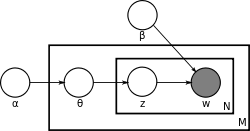
\includegraphics[width=0.55\linewidth]{lda}
	\end{minipage}
	\end{figure}\\
	$\alpha$ and $\beta$ is hyperparameters of model. 
 
    \subsection{Topic modeling as optimization problem}
	According to generative model one can estimate probability to observe collection $D$ as:
	\begin{equation} p(D) = \prod_{d \in D} \prod_{w \in d} \sum_{t} p(t|d) p(w|t) \end{equation}
	Denote $\varphi_{wt} = p(w|t)$ and $\theta_{td} = p(t|d)$. One may obtain $\varphi_{wt}$
	and $\theta_{td}$ as solution of optimization problem

	\begin{equation} \label{optimization} L = \sum_{d \in D} \sum_{w \in d} \log \sum_{t} \varphi_{wt} \theta_{td}  \to \max \end{equation}
	    with boundary
	\begin{equation} \forall t \ \ \sum_{w} \varphi_{wt} = 1, \ \ \forall d \ \ \sum_{w} \theta_{td} = 1 \end{equation}
	and
	\begin{equation} \forall t, w \ \  \varphi_{wt}  \geq 0, \ \ \forall d, t \ \ \theta_{wt}  \geq 0 \end{equation}

    \subsection{Topic modeling as matrix decomposition} \label{matrixDecomposition}

	\subsubsection{Kullback-Leibler divergence}
	    Kullback-Leibler divergence is a non-negative measure of difference between two different probability distribution:
	    \begin{equation} KL(p_i||q_i) = \sum_{i=1}^n p_i \ln\left(\frac{p_i}{q_i}\right)  \end{equation}
	    Consider an empirical distribution $\hat{p}_i$ and some parametric distribution $q_i = q_i(\alpha)$ which is used to explain $\hat{p}_i$ .
	    Easy to see that in this case minimization of KL\---divergence is equivalent to estimation of $\alpha$ by maximum-likelihood:
	    \begin{equation} KL(p_i||q_i(\alpha)) = \sum_{i=1}^n p_i \ln\left(\frac{p_i}{q_i(\alpha)}\right) \to \min_{\alpha}
	    \Leftrightarrow \sum_{i=1}^n p_i \ln(q_i(\alpha)) \to \max_{\alpha} \end{equation}

	    Thus one can easily see that (\ref{optimization}) equivalent to weighted Kullback-Leibler divergence minimization:
	    \begin{equation}
		\sum_{d \in D} n_d KL_w \left( \frac{n_{dw}}{n_d} || \sum_{t \in T} \varphi_{wt}\theta_{td} \right) \to \min_{\Phi, \Theta}
	    \end{equation}
		where $n_{wd}$\--- number of words $w$ in document $d$, $n_d$ \--- number of words in document $d$.

	\subsubsection{Matrix decomposition}
	    Denote empirical distribution of words by document as $\hat{p}(w, d) = \frac{n_{wd}}{n_d}$.
	    According to this notation one can consider the problem (\ref{optimization}) as matrix decomposition:
	    \begin{equation} F \approx_{KL} \Phi \Theta \end{equation}
	    where matrix $F = (\hat{p}(w, d))_{W \times D}$ is empirical distribution of words by document,
	    matrix $\Phi = (\varphi_{wt})_{W \times D}$ is distribution of words by topics and
	    matrix  $\Theta = (\theta_{td})_{T\times D}$ is distribution of documents by topics.
	    Thus, our optimization problem may be rewritten in Kullback–Leibler notation as
	    \begin{equation} KL(F , \Phi \Theta) \rightarrow \min \end{equation}
	    Thus PLSA may be observed as stochastic matrix decomposition.

    \subsection{Expectation\--Maximization algorithm} \label{EMAlgorithm}
	    Unfortunately (\ref{optimization}) has no analytical solution. Thus we use Expectation \-- Maximization (EM) algorithm.
	    This algorithm consists of two steps:
	    \begin{enumerate}
		\item Estimation of number $n_{dwt}$ of words $w$, produced by topic $t$ in document $d$. (E \-- step)
		\item Optimization of distribution of documents by topics and optimization of distribution of topics by words relying on
		    the $n_{dwt}$ values obtained during E \-- step . (M \-- step)
	    \end{enumerate}
	    One can estimate $n_{dwt}$ as follows:
	    \begin{equation}  n_{dwt} = n_{wd} p(w|t) p(t|d) \end{equation}
	    where $n_{wd}$ \--- number of words $w$ in document $d$.
	    Thus, probability $p(w|t)$ may be estimated as
	    \begin{equation}  p(w|t) = \frac{n_{wt}}{n_t} = \frac{\sum_d n_{dwt} }{\sum_w \sum_d n_{dwt}}   \end{equation}
	    Similarly for $p(t|d)$

    \subsection{Regularizers} \label{Regularizers}
	Regularizers may improve human-understandability of the topics, transform PLSA to LDA, provide an ability
	for semi-supervised learning (employ a prior knowledge about document topic or topics structure).
	Instead of optimization (\ref{optimization}) we optimize
	\begin{equation} \label{optimizeWithReqularizer} L(\Phi, \Theta) + R(\Phi, \Theta) \to \max_{\Phi, \Theta} \end{equation}
	Where $R(\Phi, \Theta)$ is a twice differentiable function, named regularizer.
	Solution of this problem leads to a modification of M\--step:
	\begin{equation}
	    \label{RegularizersEquation}
	    \varphi_{wt} \propto \left(\hat{n}_{wt} + \varphi_{wt} \frac{\partial  R(\Phi, \Theta)}{\partial \varphi_{wt}} \right)_+ ,\ \
	    \theta_{td} \propto \left(\hat{n}_{dt} + \theta_{td}\frac{\partial  R(\Phi, \Theta)}{\partial \theta_{td}} \right)_+
	\end{equation}
	Where $\hat{n}$ has been estimated by E\--step.

	\subsubsection{Probability interpretation}
	    Does regularizer have probabilistic interpretation? Yes, it has. Imagine that $\Phi$ and $\Theta$ have some prior distribution, for example
	    dirichlet distribution. In this case:
	    \begin{equation} \label{probabilityWithReqularizer} P(D, \Theta, \Phi) = P(D| \Theta, \Phi) \times P(\Theta, \Phi) \end{equation}
	    Logarithm equation \ref{probabilityWithReqularizer}:
	    \begin{equation} \ln P(D, \Theta, \Phi) = \ln(P(D| \Theta, \Phi) \times P(\Theta, \Phi) = \ln(P(D| \Theta, \Phi)) + \ln(P(\Theta, \Phi)) \end{equation}
	    Denote $L(\Phi, \Theta) = \ln(P(D| \Theta, \Phi))$ and $R(\Phi, \Theta) = \ln(P(\Theta, \Phi))$ and obtain \ref{optimizeWithReqularizer}

	    \paragraph{Example}
		Consider the example with symmetric dirichlet distribution\footnote{\url{http://en.wikipedia.org/wiki/Dirichlet_distribution}} with parameter $\alpha$.
		Assume we estimate $n_{td}$ for each topic in E\--step and want to perform M\-- step. We would find new distribution of document by topic as a maximum posterior probability solution:
		\begin{equation} \ln(P(\vec{\theta}| \vec{n}_{dt})) \to \max \end{equation}
		\begin{equation} \ln(P(\vec{\theta}| \vec{n}_{dt})) \propto \ln(P(\vec{n}_{dt}|\vec{\theta}) \times P(\vec{\theta})) \Leftrightarrow \end{equation}
		\begin{equation} \ln(P(\vec{\theta}| \vec{n}_{dt})) = \ln(\prod_{t \in T} \theta_t^{n_{td}} \times \prod_{t \in T}\theta_t^{\alpha - 1}) + const \Leftrightarrow  \end{equation}
		\begin{equation} \label{regularizerEquation} \ln(P(\vec{\theta}| \vec{n}_{dt})) = (\sum_{t \in T}(n_{td} + \alpha - 1) \ln(\theta_t)  + const \Leftrightarrow  \end{equation}
		And boundary:
		\begin{equation} \label{regularizerBoundary} \sum_{t \in T} \theta_t = 1 \end{equation}
		We may write down a Lagrangian from \ref{regularizerEquation} and \ref{regularizerBoundary}
		\begin{equation} L(\vec{\theta}, \lambda) = \sum_{t \in T}(n_{td} + \alpha - 1) \ln(\theta_t) - \lambda (\sum_{t \in T} \theta_t - 1)  \end{equation}
		\begin{equation} \frac{\partial L}{\partial \theta_t} = \frac{n_{td} + \alpha - 1}{\theta_t} - \lambda = 0  \end{equation}
		\begin{equation} \theta_t \propto  n_{td} + \alpha - 1 \end{equation}
		Where $n_{td}$ was estimated in E\--step and
		$\theta_{td}\frac{\partial  R(\Phi, \Theta)}{\partial \theta_{td}} = \theta_{td} \frac{\partial (\alpha - 1)\ln(\theta_{td})}{\partial \theta_{td}} = \alpha - 1 $
		is regularizer.\\
		See example of regularizer implementation in ru.ispras.modis.tm.regularizer.SymmetricDirichlet
		
		

\clearpage	\section{Quick start} \label{quickStart} In order to use topic modeling one have to perform the following step:
\begin{enumerate}
    \item Read documents
    \item Split each document into a sequence of words
    \item Replace words by it serial number
    \item Build a topic model.
    \item Train the topic model.
    \item Save results or use it in application. 
\end{enumerate}

In this section would be shown how to perform each step. 
\subsection{Read the data}
    First of all we have to read the data from disc. It worth mentioning that text normalization is non\--goal of our project, thus text should be already preprocessed. 
    This step depends on the organization of input data, so it is
    no use to describe this step in general way. Instead of this we describe this step for our example file, one may easy modify this step for his own use case. % !! криво
    In this introduction we would use file arxiv.part from directory examples. This is a thousand of scientific  papers 
    from Arxiv\footnote{\url{http://arxiv.org/}}. Texts was preprocessed, words were separated by space. Every line corresponds
    to a single document.\\
    First of all one has to read data, and split each line by space:\\
    \texttt{val lines = Source.fromFile(new File("examples/arxiv.part")).getLines()}
    \texttt{val wordsSequence = lines.map(line => line.split(" "))}\\
    Than one have to construct a TextualDocument from each sequence of words:\\
    \texttt{val textualDocuments = wordsSequence.map(words => \\  new TextualDocument(Map(DefaultAttributeType -> words)))}\\
    Each TextualDocument is a map from attribute to the correspond sequence of words. For example attribute may denote language of
    text in the case of multilingual topic modeling. 
    If there is only one attribute (as in our case) one can use \texttt{DefaultAttributeType}.  Furthermore, in such a case one can use \texttt{SingleAttributeNumerator} instead on \texttt{Numerator} -- it takes \texttt{Seq[String]} as inputes and implicitly uses \texttt{DefaultAttributeType}.
\subsection{Replace words by it serial number}
    In order to save the memory in our application we have to replace words by it serial number and group the same words together.
    $$ Seq(duck, \ \ duck, \ \ duck, \ \ goose) \to Seq((0, 3), (1, 1))) $$
    For this purpose we may use object Numerator. It takes into input sequence of textual documents, replace words by it serial number,
    group the same words and return sequence of documents. It also return Alphabet (map form word to serial number and vice versa)
    \texttt{val (documents, alphabet) = Numerator(textualDocuments)}.\\ 
    \subsubsection{How to use alphabet}
	Alphabet holds a map from words to their indices and vice versa. Thus it allow to
	\begin{enumerate}
	    \item get words by it index and attribute:\\
		\texttt{alphabet(Category, 1) // goose}
	    \item get index of word by attribute and word: \\
		\texttt{alphabet.getIndex(Category, duck) // 0}
	    \item get the number of words, corresponding to the given attribute \\
		\texttt{alphabet.numberOfWords(Category) // 100500}
	\end{enumerate}
	
\subsection{Build model}
    One can build model with class Builder (see package ru.ispras.modis.builder). Our project provides three types of builders:
    \begin{enumerate}
	\item PLSABuilder \--- builds a standard PLSA (as it is described in original paper \cite{PLSA_original})
	\item LDABuilder  \--- builds an LDA (PLSA with Dirichlet regularizer, for details section \ref{Regularizers})
	\item RobustPLSABuilder \--- builds a robust PLSA. Robust PLSA takes into account that some words are too rare and can't be explained by any topic 
	    (we call this kind of words "noise"). Some other words may be too common (for example a stop\--word, that we forget to remove in the preprocessing step). Words of this kind
	    are referred to any topic (we call that kind of word "background").  
    \end{enumerate}

    In this example we would
    use a standard PLSA, other builders work analogously.  To build plsa one should
    \begin{enumerate}
	\item Set number of topics in model: \\ \texttt{ val numberOfTopics = 25}
	\item Set the number of iterations for EM\--algorithm to perform: \\ \texttt{ val numberOfIteration = 100}
	\item Create an instance of class java.util.Random: \\     \texttt{ val random = new Random()}
	\item And build the model: \\ \texttt{ val builder = new PLSABuilder(numberOfTopics, alphabet, documents, random,  numberOfIteration)}
    \end{enumerate}

\subsection{Training a model}
    Now we build a model and can perform stochastic matrix decomposition(train the model) \\
    \texttt{val trainedModel = plsa.train(documents)}\\
    trainedModel holds the matrices $\Phi$ and $\Theta$ (see \ref{matrixDecomposition})
    $\Phi$ is distribution of words by topic thus the number in the intersects of $i\--th$ row and $j\--th$ column show the
    probability to generate word $j$ from topic $i$. Each attribute set according to the matrix $\Phi$.
    To obtain matrix $\Phi$, corresponds to attribute Category:\\
    \texttt{val phi = trainedModel.phi(Category)}\\
    $\Theta$ is a distribution of documents by topic thus the number in the intersects of $i\--th$ row and $j\--th$ column show
    the weight of topic $j$ in document $i$.
    To obtain matrix $\Theta$: \\
    \texttt{val theta = trainedModel.theta}\\

    \subsubsection{How to interpret the results}
	If you are not familiar with topic modeling read \ref{generativeModel}. In our library we store the distribution of words by topic in matrix $\Phi$,
	distribution of documents by topics in matrix $\Theta$. In order to obtain the probability to generate word $w$ from topic $t$ one may use method \\
	\texttt{trainedModel.phi(Category).probability(t, w)}\\
	In order to obtain the probability to generate topic $t$ in document $d$ \\
	\texttt{trainedModel.theta.probability(d, t)}\\
    
    \subsubsection{How to deal with matrices}
	Matrices $\Phi$ and $\Theta$ hold different information, but support the similar methods.
	Both classes hold matrix of expectation and stochastic matrix. Expectation matrix holds values, estimated by E\--step (see \ref{EMAlgorithm}),
	stochastic matrix contain a probability. Method of classes Phi and Theta are explained in table \ref{phiAndThetaMethods}
	    
	\begin{table}[ht!]
	    \caption{Method of class Phi and class Theta}
	    \label{phiAndThetaMethods}
	    \begin{tabular}{|l|p{4cm}|p{4cm} |p{4cm} |}
		\hline
		method & Phi & Theta \\
		\hline
		    addToExpectation($row$, $column$, $value$)
		    & $row$ \-- topic index column \-- word index  $column$ \-- topic index
		    & $row$ \-- document index  value \-- $n_{dwt}$  value \-- $n_{dwt}$ \\
		\hline
		    probability($rowIndex$, $columnIndex$)
		    & probability to generate word $columnIndex$ from topic $rowIndex$
		    & weight of topic $columnIndex$ in document $rowIndex$\\
		\hline
		    expectation($rowIndex$, $columnIndex$) &
		    return expected value for words, $columnIndex$ generated from topic $rowIndex$: $n_{wt}$ &
		    return expected value for words,  generated from topic $columnIndex$ in document $rowIndex$: $n_{dt}$ \\
		\hline
		    numberOfRows & number of topics & number of documents \\
		\hline
		    numberOfColumns & number of words& number of topics\\
		\hline
		dump() &\multicolumn{3}{|p{8.430cm} |}{replace negative value in expectation matrix by zero, replace value in stochastic matrix
		by corresponding values from expectation matrix, normalize stochastic matrix and replace values in expectation matrix by zero} \\ % <---- inserted &
		\hline
	    \end{tabular}
	\end{table}  
	We also have an utility to save matrix in file: \\
	\texttt{TopicHelper.saveMatrix("path/to/file", matrix)}
	where matrix may be $\Phi$ or $\Theta$. 
	One also may write top $n$ words from each topic to estimate topic coherence with 
	\texttt{TopicHelper.printAllTopics(n, phi, alphabet)}



    
    





\clearpage	\section{Building bricks of our model} \label{projectStructure} In the previous section we describe how to build a model, but we steel do not describe how model works. 
Let's fix this shortcoming. Our model support a multilingual documents, thus document may contain a few text with
different attributes, all texts in one document inherit the same distribution of topics. Thus we have had one matrix $\Phi$ per
attribute and one matrix $\Theta$ for all attribute. In order to train our model we have to
% TODO нарисовать пиздатую картинку из которой все сразу всё поймут.
\begin{enumerate}
    \item Generate some initial approximation for matrix $\Theta$ and every matrices $\Phi$
    \item \label{AlgorithmBegin} Perform E\--step and estimate the number of words $w$ in document $d$, produced by topic $t$ for every attribute.
    \item Apply reqularizer to every matrix. (see \ref{Regularizers})
    \item Perform M\--step for every matrix.
    \item Sparsify matrices $\Phi$ and matrix $\Theta$. (see \ref{sparseModel})
    \item Check the stopping criteria and return training model if it time to stop or return to the step \ref{AlgorithmBegin} otherwise.   
\end{enumerate}
\begin{figure}[!ht]
    \begin{minipage}{\textwidth}
	\includegraphics[width=1.0\linewidth]{pipeline}
    \end{minipage}
\end{figure}
The main part of our project is PLSABricks, it do the main part of work. One brick process one attribute. It performs E\--step, apples
reqularizer to matrix $\Phi$, performs M\--step to the matrix $\Phi$ and sparsifies matrix $\Phi$. PLSA include one brick per attribute,
regularizer and sparsifier for matrix $\Theta$, stopping criteria.  


\clearpage	\section{Regularizer} \label{regularizer} \subsection{Regularizer}
    The description of theory are described in \ref{Regularizers}. Hear we would describe the detail of implementation of regularizer in our project and describe some standard regularizers,
    which are implemented in our library.
    \subsubsection{Implementation}
	One may find regularizers in ru.ispras.modis.regularizer. Any regularizer should inherit from class Regularizer. In order to implement his own regularizer user have to implement methods
	regularizePhi, regularizeTheta and apply.
	\paragraph{Implementation of regularizePhi\\}
	As one may see in \ref{RegularizersEquation},
	\begin{equation} \varphi_{wt} \propto \left(\hat{n}_{wt} + \varphi_{wt} \frac{\partial  R(\Phi, \Theta)}{\partial \varphi_{wt}} \right)_+ \end{equation}
	Thus, in order to implement method regularizePhi one have to:
	\begin{itemize}
	    \item calculate $\varphi_{wt} \frac{\partial  R(\Phi, \Theta)}{\partial \varphi_{wt}}$ using matrix $\Phi$ and matrix $\Theta$ for each word $w$ and
		each topic $t$.\\
		In order to take $i$\--th row and $j$\--th column in matrix $\Phi$ one may use $$phi.probability(i, j)$$ where $i$\--- topic index,
		$j$\--- word index.\\
		Analogously for matrix $\Theta$: $$theta.probability(i, j)$$, where $i$\--topic index, $j$ \-- document index.
	    \item Add these values to matrix of expectation, in order to add $\varphi_{wt} \frac{\partial  R(\Phi, \Theta)}{\partial \varphi_{wt}}$ to
		expectation matrix $n_{wt}$ one should use method\\
		$$phi.addToExpectation(t, w, \varphi_{wt} \frac{\partial  R(\Phi, \Theta)}{\partial \varphi_{wt}})$$
	\end{itemize}
	
    \paragraph{Implementation of regularizeTheta \\}
	This method is analogous to the previous paragraph. One have to calculate $$ \theta_{td}\frac{\partial  R(\Phi, \Theta)}{\partial \varphi_{td}} $$
	and add it to expectation of $n_{dt}$.
    \paragraph{Implementation of apply \\}
	apply is used to calculate \ref{optimizeWithReqularizer} instead of log likelihood (and corresponding perplexity). If you wont calculate log likelihood or
	you are lazy to implement this method return 0f. 

    \subsubsection{Implemented reqularizer}
	Now in our project are implemented following regularizers:
	\begin{itemize}
	    \item ZeroRegularizer, it regularizer do nothing, if you don't wont to use regularizer use this one
	    \item RegularizerSum allow to apply a sequence of regularizers sequentially. For example if you have a few reqularizer: $r_1$, $r_2$, $r_3$ and you wont to
		apply them sequentially. For this aim\\
		\texttt{import ru.ispras.modis.regularizer.Regularizer.toRegularizerSum}
		\texttt{val regularizerSum = $r_1$ + $r_2$ + $r_3$}
	    \item SymmetricDirichlet, it regularizer add a dirichlet prior to the distribution of document by topic and words by topic, it is used to convert PLSA into LDA (see \ref{LDA})
 	\end{itemize}

	

\clearpage	\section{Sparsifier} \label{sparsifier} One document often corresponds to only a few topics, not to everyone. Analogously,
word corresponds only to a few topics, not to every topic. Thus some weights in
matrices $\Phi$ and $\Theta$ may be replaced by zero without drop of quality of our model. For this purpose we use
sparsifier. Any sparsifier should inherit from trait Sparsifier and implement a method apply. This method takes into input
MatrixForSparsifier and numberOfIteration. Sparsifier may obtain probabilities from matrix and decide which cells should be replaced
by zero, based on value, number of iteration and its state. To replace $i$\--th row and $j$\--th column by zero one should call\\
\texttt{matrix.setZero(i, j)}\\

\subsection{Implemented sparsifier}
    We implement
    \begin{itemize}
	\item ZeroSparsifier, it does nothing. If you don't want to use sparsifier you should use this one. 
	\item ThresholdSparsifier \-- this class replaces value with zero if it is less than threshold if it did not replaced in this way more than \texttt{maxNumberOfZeroised} during this method call and the current number of iteration exceeds \texttt{startIteration}.
    \end{itemize}



\clearpage	\section{Stopping Criteria} \label{stoppingCriteria} There is no conventional way to define how many iteration should be executed. One of the common way to do that is to execute a fixed number of
iterations, where the number of iteration is a some heuristic. There are another stopping criterion, thus we allow user to implement his own
criterion. Any criterion should inherit trait StoppingCriteria. Stopping criterion decide to stop based on perplexity after this iteration, perplexity after
previous iteration, number of iterations and internal state. 


\clearpage	\section{Multilingual topic modeling} \label{multilingual}

\bibliographystyle{unsrt}
\bibliography{userGuide} 
\end{document}
